\clearpage

\section{Comparing the Results}
\label{sec:comparing}

In this section, we will be comparing the results obtained by both the Theoretical Analysis and the Simulation.

In the following tables and plots, we can observe the results already presented in previous sections now side by side, with the first table being the result of the simulation and the second one being the result from the theoretical analysis. These are displayed in this
way as a means of easier representation.

\subsection{Table Comparison}


\begin{figure}[H]
\centering
\begin{subfigure}{.5\textwidth}
  \centering
  \begin{tabular}{|l|r|}
  \hline    
  {\bf Variable} & {\bf Value} \\ \hline
  gaindbmax & 3.834218e+01\\ \hline

  \end{tabular}
  \begin{tabular}{|l|r|}
  \hline    
  {\bf Variable} & {\bf Value} \\ \hline
  zin & 9.999982e+02,-3.99820e+02\\ \hline

 \end{tabular}
 \begin{tabular}{|l|r|}
  \hline    
  {\bf Variable} & {\bf Value} \\ \hline
  zout & 8.011868e+02,-3.99270e+02\\ \hline

  \hline
  \end{tabular}
\end{subfigure}%
\begin{subfigure}{.4\textwidth}
  \centering
  \begin{tabular}{|l|r|}
  \hline    
  {\bf Variable} & {\bf Value} \\ \hline
  gain & 8.2787e+01\\\hline gaindB & 3.8359e+01\\\hline Zire & 1.0000e+03\\\hline Ziim & -4.6904e+02\\\hline Zore & 8.1967e+02\\\hline Zoim & -3.8446e+02\\\hline 
  \end{tabular}
\end{subfigure}
\caption{Simulation Values (LEFT) and Theoretical Values (RIGHT)}
\label{fig:sbs1}
\end{figure}


\subsection{Plot Comparison}

\vspace{-3cm}

\begin{figure}[H]
\centering
\begin{subfigure}{.5\textwidth}
  \centering
  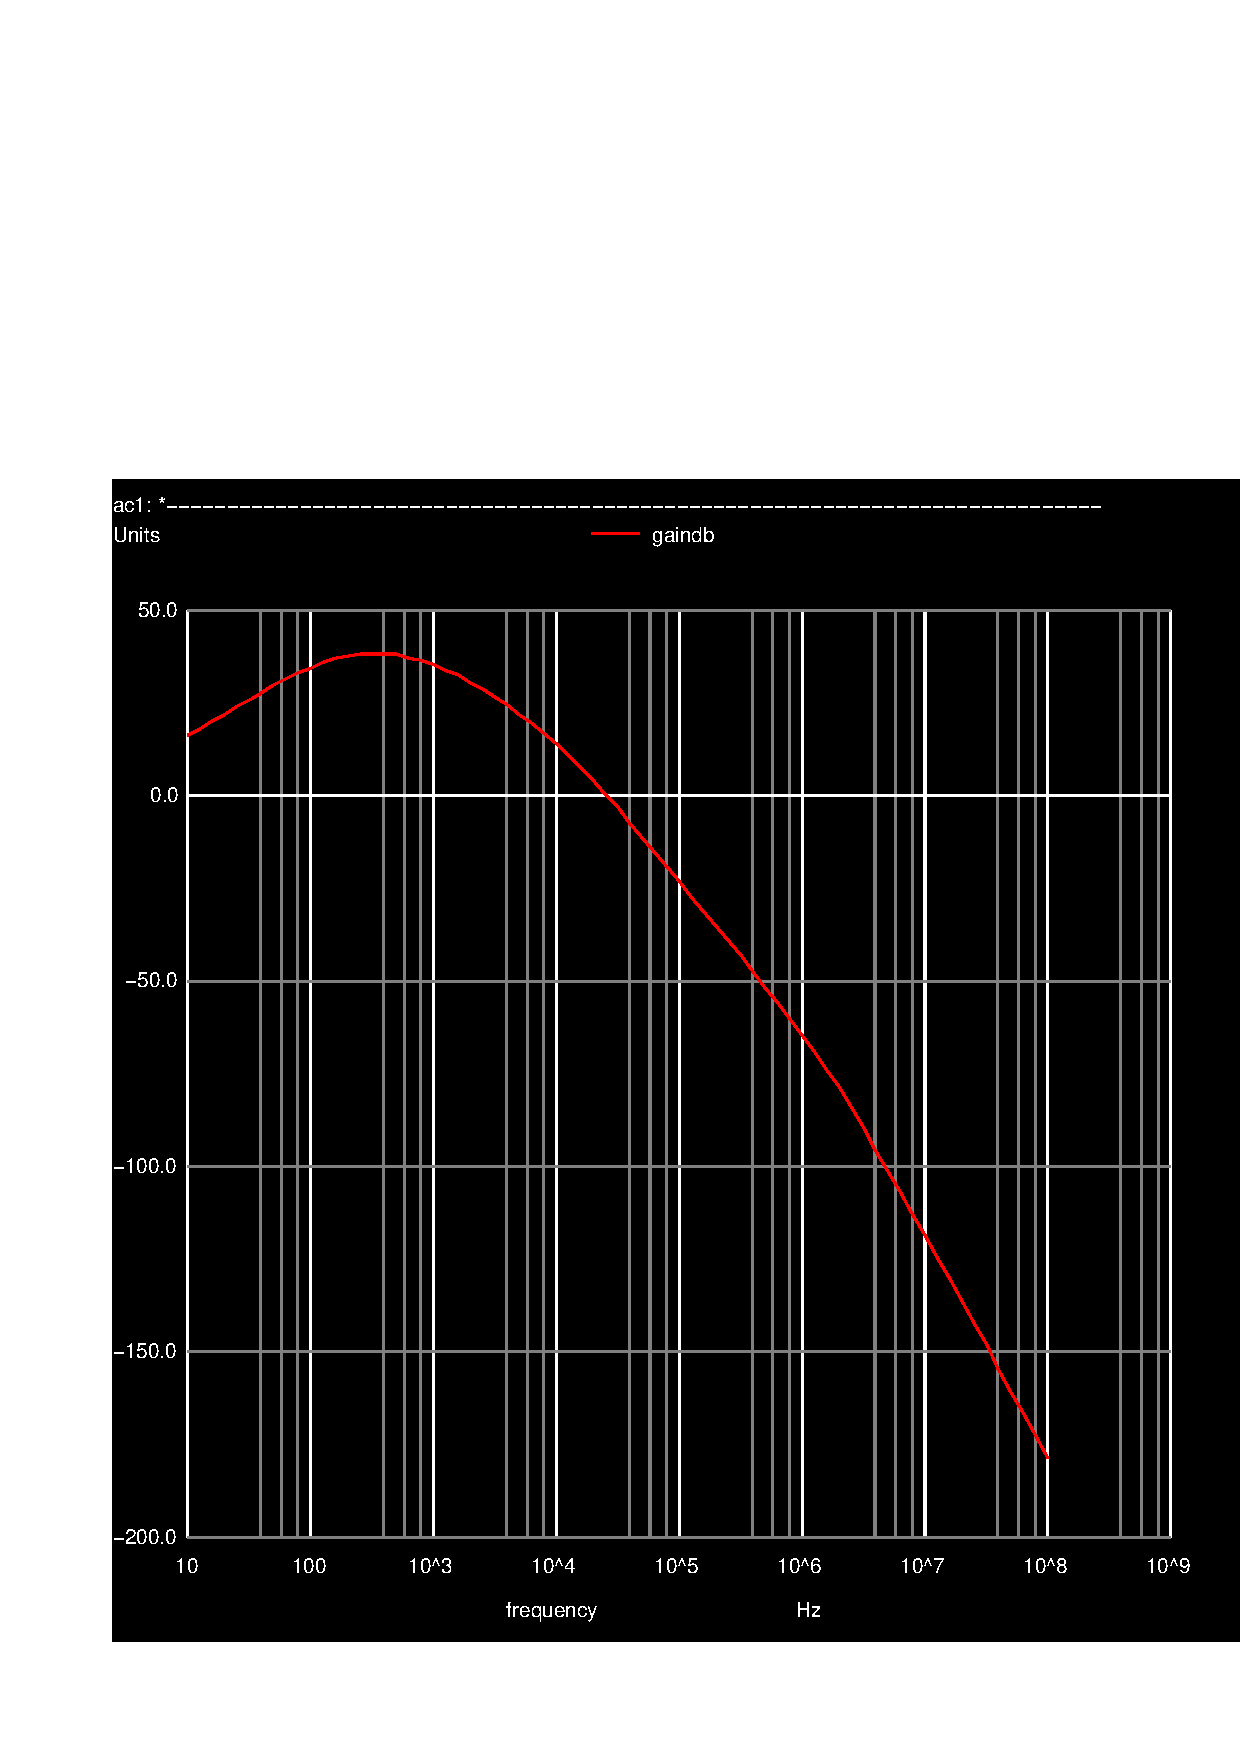
\includegraphics[width=0.9\linewidth]{../sim/gain.pdf}
\end{subfigure}%
\begin{subfigure}{.5\textwidth}
  \centering
  \vspace{3cm}
  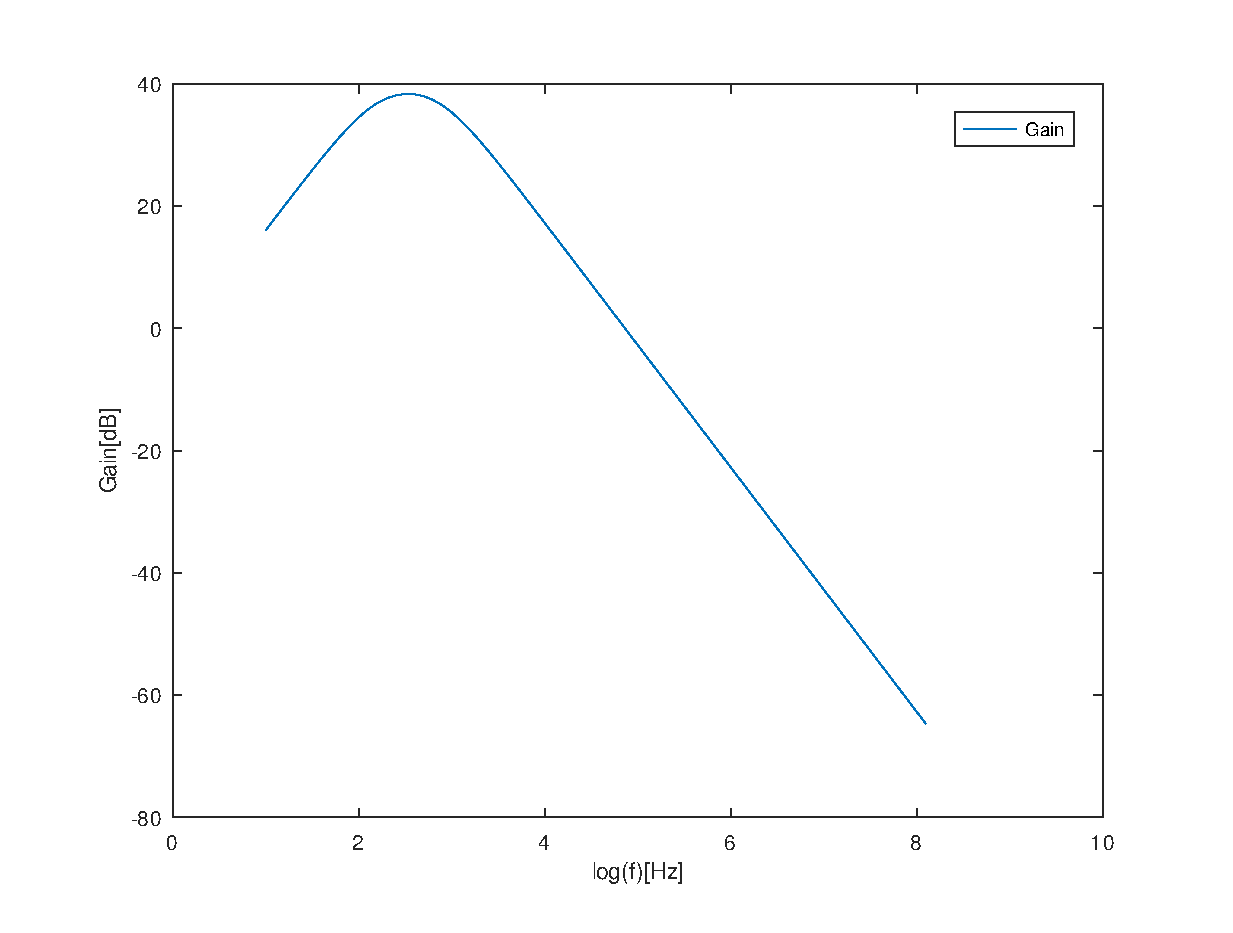
\includegraphics[width=1\linewidth]{gainteo.eps}
\end{subfigure}
\caption{Simulation Gain Values (LEFT) and Theoretial Gain Values (RIGHT)}
\label{fig:sbs3}
\end{figure}

\begin{figure}[H]
\centering
\begin{subfigure}{.5\textwidth}
  \centering
  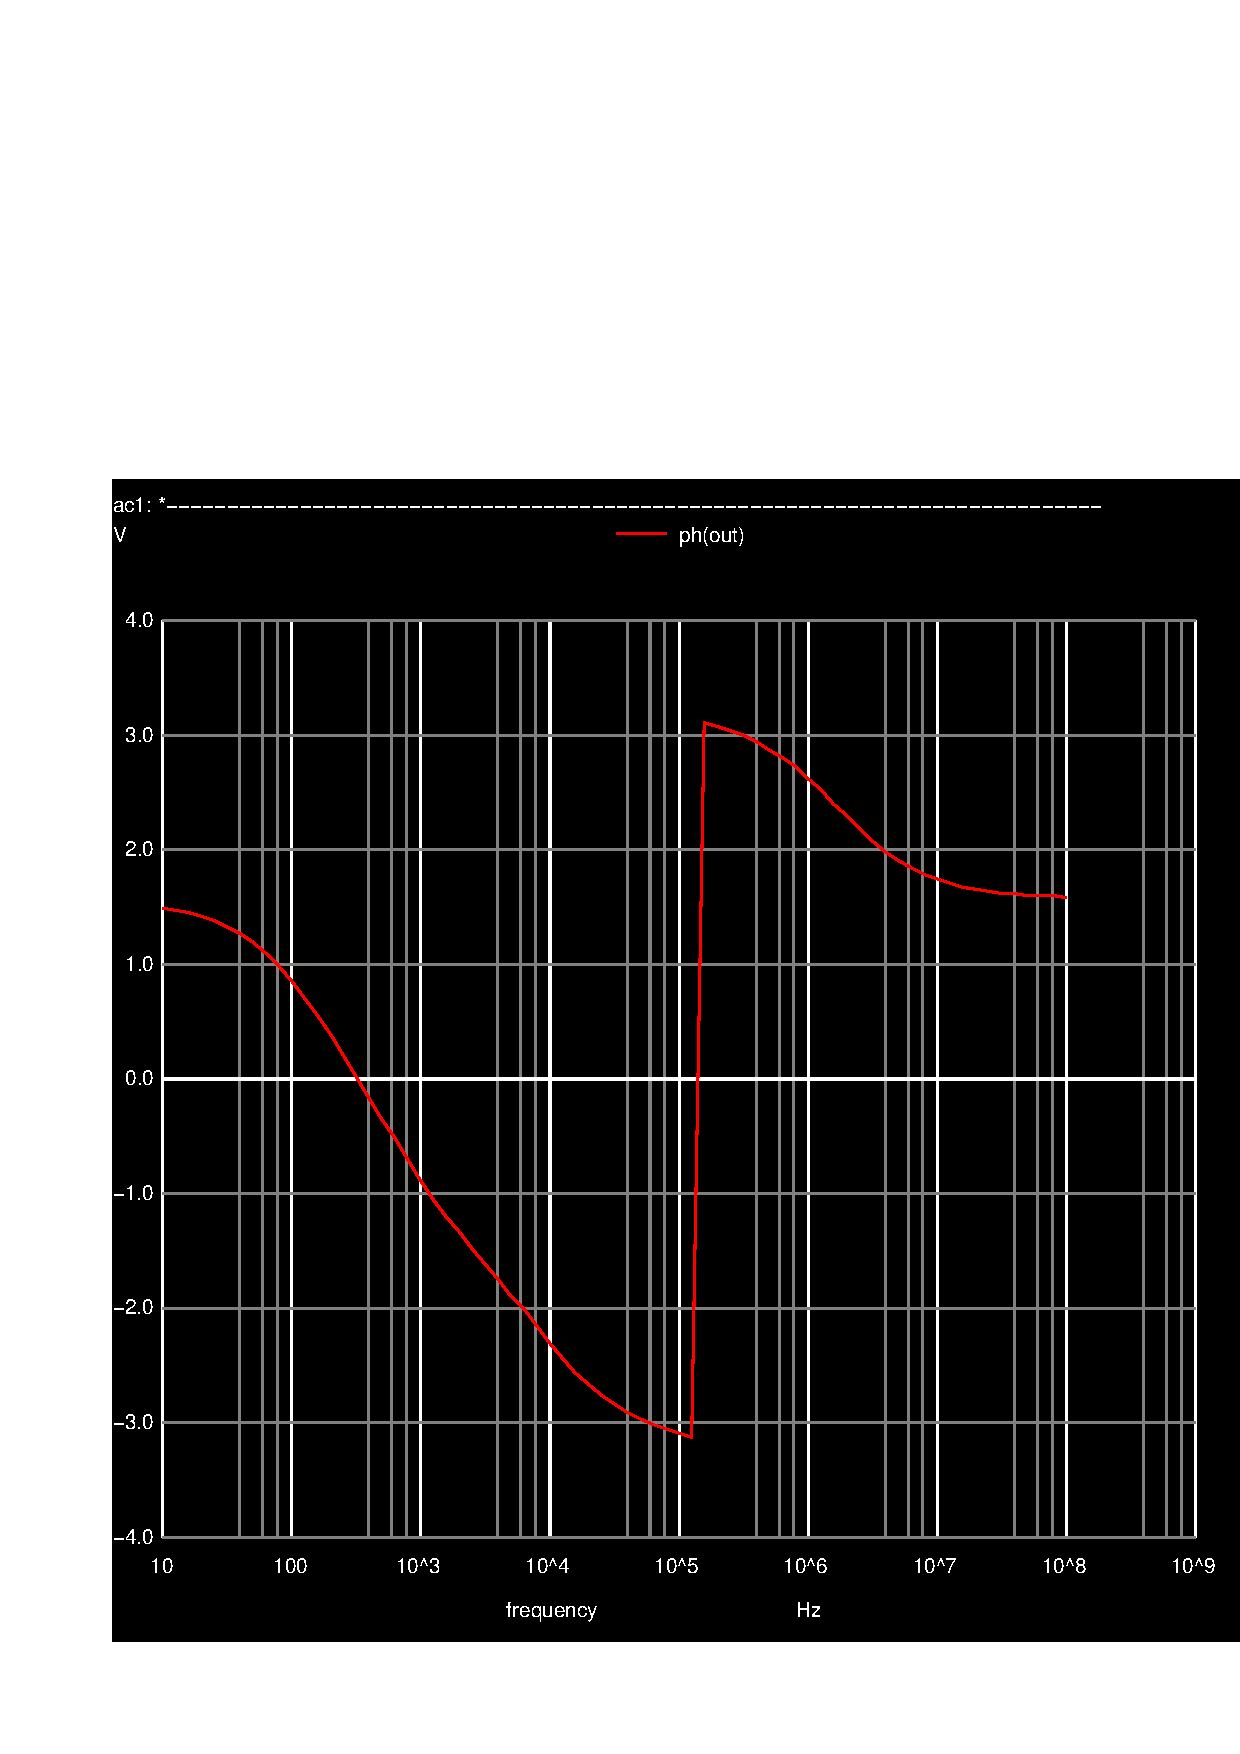
\includegraphics[width=0.9\linewidth]{../sim/phase.pdf}
\end{subfigure}%
\begin{subfigure}{.5\textwidth}
  \centering
  \vspace{3cm}
  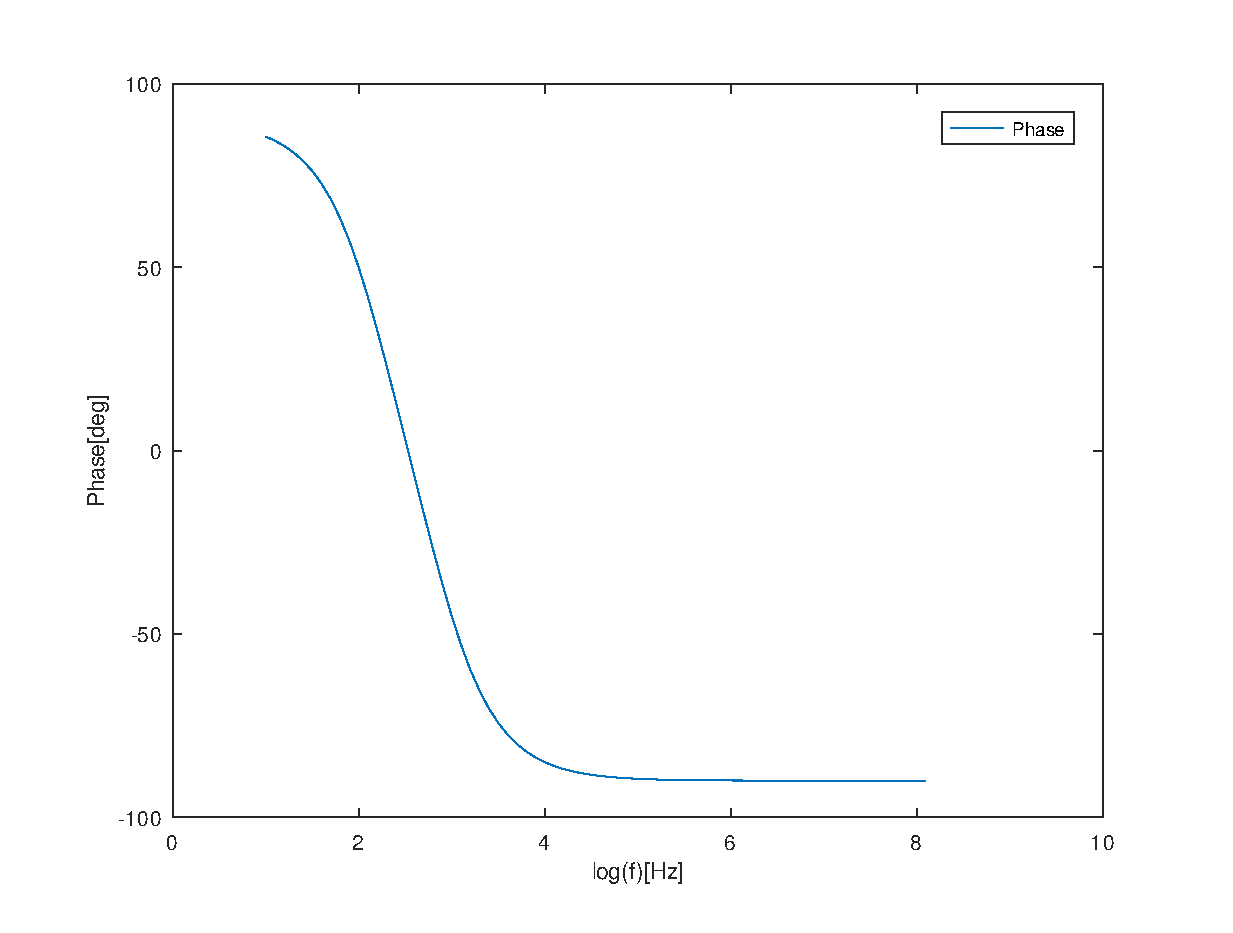
\includegraphics[width=1\linewidth]{phaseteo.eps}
\end{subfigure}
%\caption{Simulation Gain Values (LEFT) and Theoretial Gain Values (RIGHT)}
%\label{fig:sbs3}
\end{figure}